\documentclass{article}
\title{Blanchard Ch.6}
\author{Dawei Wang}
\date{\today}
\usepackage{ctex}
\usepackage{amsmath}
\usepackage{amssymb}
\usepackage{graphicx} %插入图片的宏包
\usepackage{float} %设置图片浮动位置的宏包
\usepackage{subfigure} %插入多图时用子图显示的宏包
\begin{document}
	\maketitle

\section{名义利率VS.实际利率}

以美元形式表达的利率(或更一般地,以国家货币形式表达的利率)称为名义利率(nominal interest rate)。

以一揽子商品形式表达的利率称为实际利率(real interest rate)。如果我们定义t年的实际利率为$ r_t $,那么根据定义,本年度借入一揽子商品的等价物要求在下一年度支付$ (1+r_t) $揽子商品等价物。

名义利率和实际利率的关系:我们必须调整名义利率,从而将预期的通货膨胀考虑进去。

\hspace*{\fill}

设第t年的价格水平为$ P_t $,$ i_t $为第t年的名义利率,$ P_{t+1}^e $为预期的下一年度的价格水平。则一年期的实际利率为:

\[
1+r_t=(1+i_t)\frac{P_t}{P_{t+1}^e}
\]

定义t$\sim$t+1的预期通货膨胀为$ \pi_{t+1}^e $

\[
\pi_{t+1}^e=\frac{P_{t+1}^e-P_t}{P_t}
\]

则:

\[
1+r_t=\frac{1+i_t}{1+\pi_{t+1}^e}
\]

当预期通胀率不高的时候有:

\[
r_t\simeq i_t-\pi_{t+1}^e
\]

上式的含义:

预期通胀为0时,名义利率等于实际利率;

由于预期通胀率通常为正,从而实际利率通常低于名义利率。

给定名义利率,与其通胀率越高,实际利率越低。

如果我们用CPI来度量价格水平,实际利率就告诉我们,为了现在消费更多,下一年度我们需要放弃多少消费。

\subsection{名义利率和实际利率:零利率下限和通货紧缩}

在消费者决策或者投资决策中,影响大众或者企业的是以商品形式度量的实际利率。尽管中央银行选择名义利率,但其关心的实际上是实际利率,因为它影响支出决策。因此为了实现其所希望的实际利率水平,中央银行必须将预期通货膨胀考虑进去。例如,如果中央银行希望将实际利率设定在r,它就必须选择名义利率i,从而使在给定的预期通货膨胀率$ \pi^e $下,实际利率$ r=i-\pi^e $达到其所希望的水平。

零利率下限意味着名义利率不可能为负,否则大众将不愿意持有债券。这意味着实际利率不可能低于通货膨胀率的相反数。只要预期通货膨胀利率为正,就有可能存在负的实际利率。但如果预期通货膨胀率为负,即如果大众预期通货紧缩,那么实际利率的下限就为正,并且可能变得非常高。

\section{风险和风险溢价}

风险溢价的决定因素:

违约本身的可能性。违约的可能性越高,投资者所要求的利率就越高。 

定义i为无风险债券的名义利率,i+x为风险债券(违约概率为p)的名义利率,成x为风险溢价。从而为了获得与无风险债券相同的期望回报,下面的关系式必须成立:

\[
(1+i)=(1-p)(1+i+x)+p(0)
\]

得到
\[
x=(1+i)p/(1-p)
\]

如果i和p很小,那么公式可以很好地简化为x=p。

\hspace*{\fill}

风险厌恶(risk aversion)程度。即使风险债券的期望回报等于无风险债券的期望回报,风险本身也可能使投资者不愿意持有风险债券,他们甚至会要求更高的溢价作为对风险的补偿。至于高多少,取决于投资者的风险厌恶程度。

\section{金融机构的作用}

直接融资(direct finance),最终借款者直接从最终借款提供者借入资金。

大多数借贷是通过中介机构完成的。这些金融机构从一些投资者手中获得资金,然后将这些资金出借给另一些投资者。

因为非银行实在银行的影子下成长起来的,金融体系的这一部分被称为影子银行(shadow banking)。

\subsection{杠杆率的选择}

银行的资本比率(capital ratio)定义为银行资本与资产的比率。银行的杠杆率(leverage ratio)定义为银行资产与资本的比率,即资本比率的倒数。

较高的杠杆率意味着较高的预期利润率(通过提高杠杆率,减少自有资金的投入,银行就能提高每单位资本的预期利润率),但也意味着较高的破产风险(较高的杠杆率意味着资产价值低于负债价值的风险上升,进而意味着更高的无力偿债风险insolvency)。

因此,杠杆率过低意味着利润率过低,杠杆率过高意味着破产风险过高。

\subsection{杠杆率和贷款}

若因为坏账的影响,银行虽然仍具备偿债能力,但其所面临的风险很明显高于之前。银行会打算通过要求其他投资者提供资金来增加成本,也有可能打算减少其资产负债表的规模。

\hspace*{\fill}

流动性

资产的流动性越低,大幅减价出售的风险越高,银行丧失偿债能力进而破产的风险也越高。负债的流动性越高(即投资者要求收回资金的难度越低),大幅减价出售的风险就越高,银行丧失偿债能力进而破产的风险也越高。

\section{扩展IS-LM模型}

首先区分名义利率和实际利率。其次,必须区分中央银行决定的利率和借款者实际面临的利率。这些利率即取决于与借款者相关的风险,又取决于金融中介的健康状况。风险越高,或者金融中介的杠杆率越高,借款者需要支付的利率就越高。

IS关系:

\[
Y=C(Y-T)+I(Y,i-\pi^e+x)+G
\]

LM关系:

\[
i=\overline{i}
\]

LM关系没有变。中央银行仍然控制名义利率。但是IS关系发生了两个变化:出现了预期通货膨胀$ \pi^e $,出现了风险溢价x。

预期通货膨胀反映了如下事实:在其他条件不变的情况下,支出决策取决于实际利率$ r=i-\pi^e $,而非名义利率。

这两个等式清楚地表明,进入LM关系的利率不再是进入IS关系的利率r+x。

我们把进入LM关系式的利率称为(名义)政策利率(policy rate,因为它是由货币政策决定的利率),将进入IS关系式的利率称为(实际)借款利率(borrowing rate,因为它是消费者和企业能够获得借款的利率)。

尽管中央银行正式地选择名义利率,但实际上它可以通过实现其所希望地实际利率水平的方式来选择它。因此,我们可以认为中央银行直接选择实际利率,并将上述两个等式改写为:

\[
IS\enspace relationship: Y=C(Y-T)+I(Y,r+x)+G
\]

\[
LM\enspace relationship: r=\overline{r}
\]

中央银行选择实际政策利率r。但是与支出决策相关的实际利率是借款利率r+x它不仅取决于政策利率,还取决于风险溢价。

\begin{figure}[H] %H为当前位置,!htb为忽略美学标准,htbp为浮动图形
	\centering %图片居中
	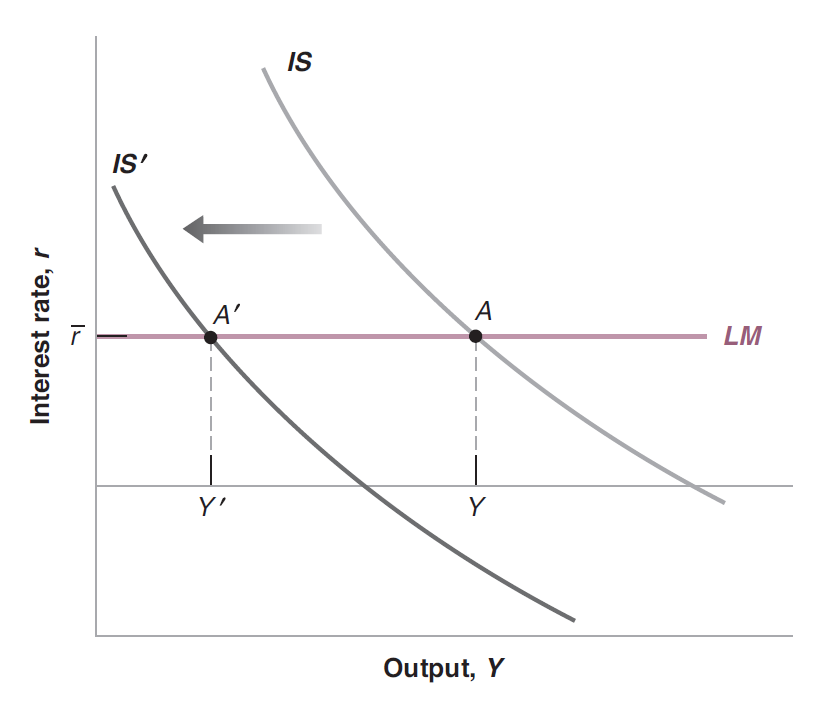
\includegraphics[width=1\textwidth]{6_1} %插入图片,[]中设置图片大小,{}中是图片文件名
	\caption{Financial Shocks
		and Output} %最终文档中希望显示的图片标题
	\label{Fig.main2} %用于文内引用的标签
\end{figure}

纵轴度量实际政策利率,横轴度量产出。IS曲线根据给定的G、T和x画出。在其他条件不变的情况下,实际政策利率上升,支出下降,进而产出下降:IS曲线向下倾斜。LM曲线是一条位于政策利率之上(中央银行选择的实际利率)的水平线。均衡点由A点给出,对应产出水平Y。

P.S.:x增加,IS曲线向左移动,均衡产出下降。

\hspace*{\fill}

能够使需求增加足够的量,并使产出恢复到其初始水平的政策利率很可能是负的。


由于名义利率下限的存在,使中央银行能够实现的最低实际利率为$ r=i-\pi^e=0-\pi^e=-\pi^e $。因此名义利率下限的存在限制了中央银行使用货币政策的操作空间。




















\end{document}